\documentclass[1p]{elsarticle_modified}
%\bibliographystyle{elsarticle-num}

%\usepackage[colorlinks]{hyperref}
%\usepackage{abbrmath_seonhwa} %\Abb, \Ascr, \Acal ,\Abf, \Afrak
\usepackage{amsfonts}
\usepackage{amssymb}
\usepackage{amsmath}
\usepackage{amsthm}
\usepackage{scalefnt}
\usepackage{amsbsy}
\usepackage{kotex}
\usepackage{caption}
\usepackage{subfig}
\usepackage{color}
\usepackage{graphicx}
\usepackage{xcolor} %% white, black, red, green, blue, cyan, magenta, yellow
\usepackage{float}
\usepackage{setspace}
\usepackage{hyperref}

\usepackage{tikz}
\usetikzlibrary{arrows}

\usepackage{multirow}
\usepackage{array} % fixed length table
\usepackage{hhline}

%%%%%%%%%%%%%%%%%%%%%
\makeatletter
\renewcommand*\env@matrix[1][\arraystretch]{%
	\edef\arraystretch{#1}%
	\hskip -\arraycolsep
	\let\@ifnextchar\new@ifnextchar
	\array{*\c@MaxMatrixCols c}}
\makeatother %https://tex.stackexchange.com/questions/14071/how-can-i-increase-the-line-spacing-in-a-matrix
%%%%%%%%%%%%%%%

\usepackage[normalem]{ulem}

\newcommand{\msout}[1]{\ifmmode\text{\sout{\ensuremath{#1}}}\else\sout{#1}\fi}
%SOURCE: \msout is \stkout macro in https://tex.stackexchange.com/questions/20609/strikeout-in-math-mode

\newcommand{\cancel}[1]{
	\ifmmode
	{\color{red}\msout{#1}}
	\else
	{\color{red}\sout{#1}}
	\fi
}

\newcommand{\add}[1]{
	{\color{blue}\uwave{#1}}
}

\newcommand{\replace}[2]{
	\ifmmode
	{\color{red}\msout{#1}}{\color{blue}\uwave{#2}}
	\else
	{\color{red}\sout{#1}}{\color{blue}\uwave{#2}}
	\fi
}

\newcommand{\Sol}{\mathcal{S}} %segment
\newcommand{\D}{D} %diagram
\newcommand{\A}{\mathcal{A}} %arc


%%%%%%%%%%%%%%%%%%%%%%%%%%%%%5 test

\def\sl{\operatorname{\textup{SL}}(2,\Cbb)}
\def\psl{\operatorname{\textup{PSL}}(2,\Cbb)}
\def\quan{\mkern 1mu \triangleright \mkern 1mu}

\theoremstyle{definition}
\newtheorem{thm}{Theorem}[section]
\newtheorem{prop}[thm]{Proposition}
\newtheorem{lem}[thm]{Lemma}
\newtheorem{ques}[thm]{Question}
\newtheorem{cor}[thm]{Corollary}
\newtheorem{defn}[thm]{Definition}
\newtheorem{exam}[thm]{Example}
\newtheorem{rmk}[thm]{Remark}
\newtheorem{alg}[thm]{Algorithm}

\newcommand{\I}{\sqrt{-1}}
\begin{document}

%\begin{frontmatter}
%
%\title{Boundary parabolic representations of knots up to 8 crossings}
%
%%% Group authors per affiliation:
%\author{Yunhi Cho} 
%\address{Department of Mathematics, University of Seoul, Seoul, Korea}
%\ead{yhcho@uos.ac.kr}
%
%
%\author{Seonhwa Kim} %\fnref{s_kim}}
%\address{Center for Geometry and Physics, Institute for Basic Science, Pohang, 37673, Korea}
%\ead{ryeona17@ibs.re.kr}
%
%\author{Hyuk Kim}
%\address{Department of Mathematical Sciences, Seoul National University, Seoul 08826, Korea}
%\ead{hyukkim@snu.ac.kr}
%
%\author{Seokbeom Yoon}
%\address{Department of Mathematical Sciences, Seoul National University, Seoul, 08826,  Korea}
%\ead{sbyoon15@snu.ac.kr}
%
%\begin{abstract}
%We find all boundary parabolic representation of knots up to 8 crossings.
%
%\end{abstract}
%\begin{keyword}
%    \MSC[2010] 57M25 
%\end{keyword}
%
%\end{frontmatter}

%\linenumbers
%\tableofcontents
%
\newcommand\colored[1]{\textcolor{white}{\rule[-0.35ex]{0.8em}{1.4ex}}\kern-0.8em\color{red} #1}%
%\newcommand\colored[1]{\textcolor{white}{ #1}\kern-2.17ex	\textcolor{white}{ #1}\kern-1.81ex	\textcolor{white}{ #1}\kern-2.15ex\color{red}#1	}

{\Large $\underline{12n_{0392}~(K12n_{0392})}$}

\setlength{\tabcolsep}{10pt}
\renewcommand{\arraystretch}{1.6}
\vspace{1cm}\begin{tabular}{m{100pt}>{\centering\arraybackslash}m{274pt}}
\multirow{5}{120pt}{
	\centering
	\includegraphics[width=112pt]{../../../GIT/diagram.site/Diagrams/png/2481_12n_0392.png}\\
\ \ \ A knot diagram\footnotemark}&
\allowdisplaybreaks
\textbf{Linearized knot diagam} \\
\cline{2-2}
 &
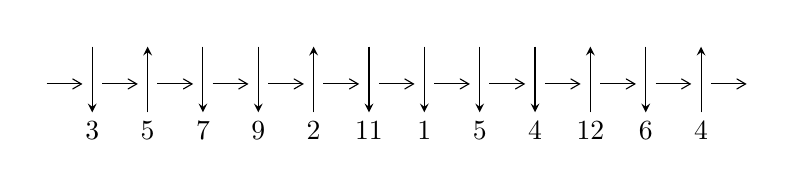
\begin{tikzpicture}[x=20pt, y=17pt]
	% nodes
	\node (C0) at (0, 0) {};
	\node (C1) at (1, 0) {};
	\node (C1U) at (1, +1) {};
	\node (C1D) at (1, -1) {3};

	\node (C2) at (2, 0) {};
	\node (C2U) at (2, +1) {};
	\node (C2D) at (2, -1) {5};

	\node (C3) at (3, 0) {};
	\node (C3U) at (3, +1) {};
	\node (C3D) at (3, -1) {7};

	\node (C4) at (4, 0) {};
	\node (C4U) at (4, +1) {};
	\node (C4D) at (4, -1) {9};

	\node (C5) at (5, 0) {};
	\node (C5U) at (5, +1) {};
	\node (C5D) at (5, -1) {2};

	\node (C6) at (6, 0) {};
	\node (C6U) at (6, +1) {};
	\node (C6D) at (6, -1) {11};

	\node (C7) at (7, 0) {};
	\node (C7U) at (7, +1) {};
	\node (C7D) at (7, -1) {1};

	\node (C8) at (8, 0) {};
	\node (C8U) at (8, +1) {};
	\node (C8D) at (8, -1) {5};

	\node (C9) at (9, 0) {};
	\node (C9U) at (9, +1) {};
	\node (C9D) at (9, -1) {4};

	\node (C10) at (10, 0) {};
	\node (C10U) at (10, +1) {};
	\node (C10D) at (10, -1) {12};

	\node (C11) at (11, 0) {};
	\node (C11U) at (11, +1) {};
	\node (C11D) at (11, -1) {6};

	\node (C12) at (12, 0) {};
	\node (C12U) at (12, +1) {};
	\node (C12D) at (12, -1) {4};
	\node (C13) at (13, 0) {};

	% arrows
	\draw[->,>={angle 60}]
	(C0) edge (C1) (C1) edge (C2) (C2) edge (C3) (C3) edge (C4) (C4) edge (C5) (C5) edge (C6) (C6) edge (C7) (C7) edge (C8) (C8) edge (C9) (C9) edge (C10) (C10) edge (C11) (C11) edge (C12) (C12) edge (C13) ;	\draw[->,>=stealth]
	(C1U) edge (C1D) (C2D) edge (C2U) (C3U) edge (C3D) (C4U) edge (C4D) (C5D) edge (C5U) (C6U) edge (C6D) (C7U) edge (C7D) (C8U) edge (C8D) (C9U) edge (C9D) (C10D) edge (C10U) (C11U) edge (C11D) (C12D) edge (C12U) ;
	\end{tikzpicture} \\
\hhline{~~} \\& 
\textbf{Solving Sequence} \\ \cline{2-2} 
 &
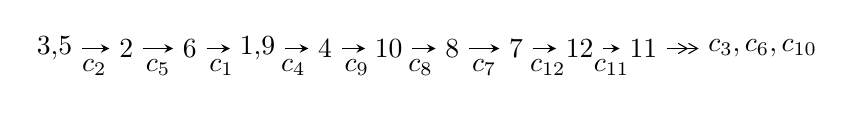
\begin{tikzpicture}[x=23pt, y=7pt]
	% node
	\node (A0) at (-1/8, 0) {3,5};
	\node (A1) at (1, 0) {2};
	\node (A2) at (2, 0) {6};
	\node (A3) at (49/16, 0) {1,9};
	\node (A4) at (33/8, 0) {4};
	\node (A5) at (41/8, 0) {10};
	\node (A6) at (49/8, 0) {8};
	\node (A7) at (57/8, 0) {7};
	\node (A8) at (65/8, 0) {12};
	\node (A9) at (73/8, 0) {11};
	\node (C1) at (1/2, -1) {$c_{2}$};
	\node (C2) at (3/2, -1) {$c_{5}$};
	\node (C3) at (5/2, -1) {$c_{1}$};
	\node (C4) at (29/8, -1) {$c_{4}$};
	\node (C5) at (37/8, -1) {$c_{9}$};
	\node (C6) at (45/8, -1) {$c_{8}$};
	\node (C7) at (53/8, -1) {$c_{7}$};
	\node (C8) at (61/8, -1) {$c_{12}$};
	\node (C9) at (69/8, -1) {$c_{11}$};
	\node (A10) at (11, 0) {$c_{3},c_{6},c_{10}$};

	% edge
	\draw[->,>=stealth]	
	(A0) edge (A1) (A1) edge (A2) (A2) edge (A3) (A3) edge (A4) (A4) edge (A5) (A5) edge (A6) (A6) edge (A7) (A7) edge (A8) (A8) edge (A9) ;
	\draw[->>,>={angle 60}]	
	(A9) edge (A10);
\end{tikzpicture} \\ 

\end{tabular} \\

\footnotetext{
The image of knot diagram is generated by the software ``\textbf{Draw programme}" developed by Andrew Bartholomew(\url{http://www.layer8.co.uk/maths/draw/index.htm\#Running-draw}), where we modified some parts for our purpose(\url{https://github.com/CATsTAILs/LinksPainter}).
}\phantom \\ \newline 
\centering \textbf{Ideals for irreducible components\footnotemark of $X_{\text{par}}$} 
 
\begin{align*}
I^u_{1}&=\langle 
-18 u^{26}+125 u^{25}+\cdots+4 b-220,\;-9 u^{26}+43 u^{25}+\cdots+16 a+312,\;u^{27}-7 u^{26}+\cdots+128 u-16\rangle \\
I^u_{2}&=\langle 
22944250 a^7 u^4-33783291 a^6 u^4+\cdots+121889135 a+78299476,\;2 a^6 u^4- a^5 u^4+\cdots-13 a+5,\\
\phantom{I^u_{2}}&\phantom{= \langle  }u^5+u^4+2 u^3+u^2+u+1\rangle \\
I^u_{3}&=\langle 
2 u^{17}+4 u^{16}+\cdots+b+3,\;u^{17}+4 u^{16}+\cdots+2 a-1,\;u^{18}+2 u^{17}+\cdots+u+2\rangle \\
\\
\end{align*}
\raggedright * 3 irreducible components of $\dim_{\mathbb{C}}=0$, with total 85 representations.\\
\footnotetext{All coefficients of polynomials are rational numbers. But the coefficients are sometimes approximated in decimal forms when there is not enough margin.}
\newpage
\renewcommand{\arraystretch}{1}
\centering \section*{I. $I^u_{1}= \langle -18 u^{26}+125 u^{25}+\cdots+4 b-220,\;-9 u^{26}+43 u^{25}+\cdots+16 a+312,\;u^{27}-7 u^{26}+\cdots+128 u-16 \rangle$}
\flushleft \textbf{(i) Arc colorings}\\
\begin{tabular}{m{7pt} m{180pt} m{7pt} m{180pt} }
\flushright $a_{3}=$&$\begin{pmatrix}1\\0\end{pmatrix}$ \\
\flushright $a_{5}=$&$\begin{pmatrix}0\\u\end{pmatrix}$ \\
\flushright $a_{2}=$&$\begin{pmatrix}1\\u^2\end{pmatrix}$ \\
\flushright $a_{6}=$&$\begin{pmatrix}u\\u^3+u\end{pmatrix}$ \\
\flushright $a_{1}=$&$\begin{pmatrix}u^2+1\\u^2\end{pmatrix}$ \\
\flushright $a_{9}=$&$\begin{pmatrix}0.562500 u^{26}-2.68750 u^{25}+\cdots+128.250 u-19.5000\\\frac{9}{2} u^{26}-\frac{125}{4} u^{25}+\cdots-\frac{903}{2} u+55\end{pmatrix}$ \\
\flushright $a_{4}=$&$\begin{pmatrix}\frac{9}{16} u^{26}-\frac{57}{16} u^{25}+\cdots-\frac{135}{2} u+10\\\frac{3}{8} u^{26}-\frac{19}{8} u^{25}+\cdots-62 u+9\end{pmatrix}$ \\
\flushright $a_{10}=$&$\begin{pmatrix}\frac{75}{16} u^{26}-\frac{349}{16} u^{25}+\cdots-\frac{1055}{4} u+42\\\frac{57}{4} u^{26}-\frac{333}{4} u^{25}+\cdots-918 u+121\end{pmatrix}$ \\
\flushright $a_{8}=$&$\begin{pmatrix}0.562500 u^{26}-2.68750 u^{25}+\cdots+128.250 u-19.5000\\\frac{21}{4} u^{26}-33 u^{25}+\cdots-\frac{601}{2} u+35\end{pmatrix}$ \\
\flushright $a_{7}=$&$\begin{pmatrix}-3.43750 u^{26}+19.5625 u^{25}+\cdots-25.2500 u+11.5000\\-\frac{5}{4} u^{26}+\frac{19}{2} u^{25}+\cdots+\frac{183}{2} u-9\end{pmatrix}$ \\
\flushright $a_{12}=$&$\begin{pmatrix}2.12500 u^{26}-11.7500 u^{25}+\cdots-299.750 u+46.5000\\\frac{25}{8} u^{26}-\frac{135}{8} u^{25}+\cdots-\frac{453}{2} u+34\end{pmatrix}$ \\
\flushright $a_{11}=$&$\begin{pmatrix}\frac{13}{8} u^{26}-\frac{35}{4} u^{25}+\cdots-\frac{111}{4} u+\frac{9}{2}\\-\frac{11}{8} u^{26}+\frac{57}{8} u^{25}+\cdots+\frac{203}{2} u-16\end{pmatrix}$\\&\end{tabular}
\flushleft \textbf{(ii) Obstruction class $= -1$}\\~\\
\flushleft \textbf{(iii) Cusp Shapes $= -\frac{5}{2} u^{26}+\frac{27}{2} u^{25}+\cdots+66 u-18$}\\~\\
\newpage\renewcommand{\arraystretch}{1}
\flushleft \textbf{(iv) u-Polynomials at the component}\newline \\
\begin{tabular}{m{50pt}|m{274pt}}
Crossings & \hspace{64pt}u-Polynomials at each crossing \\
\hline $$\begin{aligned}c_{1}\end{aligned}$$&$\begin{aligned}
&u^{27}+13 u^{26}+\cdots+640 u-256
\end{aligned}$\\
\hline $$\begin{aligned}c_{2},c_{5}\end{aligned}$$&$\begin{aligned}
&u^{27}+7 u^{26}+\cdots+128 u+16
\end{aligned}$\\
\hline $$\begin{aligned}c_{3},c_{4},c_{8}\\c_{9}\end{aligned}$$&$\begin{aligned}
&u^{27}- u^{24}+\cdots+u+1
\end{aligned}$\\
\hline $$\begin{aligned}c_{6},c_{11}\end{aligned}$$&$\begin{aligned}
&u^{27}-9 u^{26}+\cdots-176 u+32
\end{aligned}$\\
\hline $$\begin{aligned}c_{7}\end{aligned}$$&$\begin{aligned}
&u^{27}-2 u^{26}+\cdots+3 u+1
\end{aligned}$\\
\hline $$\begin{aligned}c_{10}\end{aligned}$$&$\begin{aligned}
&u^{27}-9 u^{26}+\cdots+768 u+1024
\end{aligned}$\\
\hline $$\begin{aligned}c_{12}\end{aligned}$$&$\begin{aligned}
&u^{27}+2 u^{26}+\cdots+u+1
\end{aligned}$\\
\hline
\end{tabular}\\~\\
\newpage\renewcommand{\arraystretch}{1}
\flushleft \textbf{(v) Riley Polynomials at the component}\newline \\
\begin{tabular}{m{50pt}|m{274pt}}
Crossings & \hspace{64pt}Riley Polynomials at each crossing \\
\hline $$\begin{aligned}c_{1}\end{aligned}$$&$\begin{aligned}
&y^{27}+y^{26}+\cdots+1384448 y-65536
\end{aligned}$\\
\hline $$\begin{aligned}c_{2},c_{5}\end{aligned}$$&$\begin{aligned}
&y^{27}+13 y^{26}+\cdots+640 y-256
\end{aligned}$\\
\hline $$\begin{aligned}c_{3},c_{4},c_{8}\\c_{9}\end{aligned}$$&$\begin{aligned}
&y^{27}+26 y^{25}+\cdots-5 y-1
\end{aligned}$\\
\hline $$\begin{aligned}c_{6},c_{11}\end{aligned}$$&$\begin{aligned}
&y^{27}+9 y^{26}+\cdots+768 y-1024
\end{aligned}$\\
\hline $$\begin{aligned}c_{7}\end{aligned}$$&$\begin{aligned}
&y^{27}-28 y^{26}+\cdots-33 y-1
\end{aligned}$\\
\hline $$\begin{aligned}c_{10}\end{aligned}$$&$\begin{aligned}
&y^{27}+17 y^{26}+\cdots+196608 y-1048576
\end{aligned}$\\
\hline $$\begin{aligned}c_{12}\end{aligned}$$&$\begin{aligned}
&y^{27}+44 y^{26}+\cdots+43 y-1
\end{aligned}$\\
\hline
\end{tabular}\\~\\
\newpage\flushleft \textbf{(vi) Complex Volumes and Cusp Shapes}
$$\begin{array}{c|c|c}  
\text{Solutions to }I^u_{1}& \I (\text{vol} + \sqrt{-1}CS) & \text{Cusp shape}\\
 \hline 
\begin{aligned}
u &= \phantom{-}0.105020 + 1.000790 I \\
a &= \phantom{-}0.488571 - 0.501972 I \\
b &= -0.442028 - 0.586779 I\end{aligned}
 & -1.48211 - 1.37107 I & -5.86313 + 4.22011 I \\ \hline\begin{aligned}
u &= \phantom{-}0.105020 - 1.000790 I \\
a &= \phantom{-}0.488571 + 0.501972 I \\
b &= -0.442028 + 0.586779 I\end{aligned}
 & -1.48211 + 1.37107 I & -5.86313 - 4.22011 I \\ \hline\begin{aligned}
u &= \phantom{-}0.960149 + 0.220645 I \\
a &= -1.19030 - 0.88560 I \\
b &= -0.40669 - 1.51529 I\end{aligned}
 & -3.42062 - 10.51250 I & -2.02610 + 6.29525 I \\ \hline\begin{aligned}
u &= \phantom{-}0.960149 - 0.220645 I \\
a &= -1.19030 + 0.88560 I \\
b &= -0.40669 + 1.51529 I\end{aligned}
 & -3.42062 + 10.51250 I & -2.02610 - 6.29525 I \\ \hline\begin{aligned}
u &= -0.914332 + 0.494714 I \\
a &= -0.185333 + 0.579265 I \\
b &= \phantom{-}0.383928 + 0.944693 I\end{aligned}
 & \phantom{-}3.55128 + 0.44727 I & \phantom{-}1.70598 + 5.83861 I \\ \hline\begin{aligned}
u &= -0.914332 - 0.494714 I \\
a &= -0.185333 - 0.579265 I \\
b &= \phantom{-}0.383928 - 0.944693 I\end{aligned}
 & \phantom{-}3.55128 - 0.44727 I & \phantom{-}1.70598 - 5.83861 I \\ \hline\begin{aligned}
u &= -0.567653 + 0.888742 I \\
a &= \phantom{-}0.362550 - 0.525693 I \\
b &= -0.627644 - 0.668484 I\end{aligned}
 & -0.19746 - 2.14437 I & -2.39759 + 4.10548 I \\ \hline\begin{aligned}
u &= -0.567653 - 0.888742 I \\
a &= \phantom{-}0.362550 + 0.525693 I \\
b &= -0.627644 + 0.668484 I\end{aligned}
 & -0.19746 + 2.14437 I & -2.39759 - 4.10548 I \\ \hline\begin{aligned}
u &= \phantom{-}0.907665 + 0.211669 I \\
a &= \phantom{-}1.28828 + 0.73242 I \\
b &= \phantom{-}0.427679 + 1.271000 I\end{aligned}
 & -4.63592 - 4.02746 I & -3.88519 + 2.04862 I \\ \hline\begin{aligned}
u &= \phantom{-}0.907665 - 0.211669 I \\
a &= \phantom{-}1.28828 - 0.73242 I \\
b &= \phantom{-}0.427679 - 1.271000 I\end{aligned}
 & -4.63592 + 4.02746 I & -3.88519 - 2.04862 I\\
 \hline 
 \end{array}$$\newpage$$\begin{array}{c|c|c}  
\text{Solutions to }I^u_{1}& \I (\text{vol} + \sqrt{-1}CS) & \text{Cusp shape}\\
 \hline 
\begin{aligned}
u &= \phantom{-}0.782200 + 0.463303 I \\
a &= -0.855769 - 0.381199 I \\
b &= \phantom{-}0.482293 - 1.128990 I\end{aligned}
 & \phantom{-}3.60283 - 2.96457 I & \phantom{-}0.31391 + 6.24123 I \\ \hline\begin{aligned}
u &= \phantom{-}0.782200 - 0.463303 I \\
a &= -0.855769 + 0.381199 I \\
b &= \phantom{-}0.482293 + 1.128990 I\end{aligned}
 & \phantom{-}3.60283 + 2.96457 I & \phantom{-}0.31391 - 6.24123 I \\ \hline\begin{aligned}
u &= \phantom{-}0.430772 + 1.068380 I \\
a &= -0.168300 + 0.664974 I \\
b &= -0.42525 + 1.51993 I\end{aligned}
 & -3.69679 + 3.48476 I & -13.31039 - 2.89782 I \\ \hline\begin{aligned}
u &= \phantom{-}0.430772 - 1.068380 I \\
a &= -0.168300 - 0.664974 I \\
b &= -0.42525 - 1.51993 I\end{aligned}
 & -3.69679 - 3.48476 I & -13.31039 + 2.89782 I \\ \hline\begin{aligned}
u &= \phantom{-}0.610468 + 1.088930 I \\
a &= -0.267324 - 0.684625 I \\
b &= \phantom{-}1.07720 - 1.97646 I\end{aligned}
 & \phantom{-}1.72849 + 8.21568 I & -1.80289 - 11.79925 I \\ \hline\begin{aligned}
u &= \phantom{-}0.610468 - 1.088930 I \\
a &= -0.267324 + 0.684625 I \\
b &= \phantom{-}1.07720 + 1.97646 I\end{aligned}
 & \phantom{-}1.72849 - 8.21568 I & -1.80289 + 11.79925 I \\ \hline\begin{aligned}
u &= -0.812166 + 1.037250 I \\
a &= -0.307751 + 0.460402 I \\
b &= \phantom{-}0.775885 + 0.808103 I\end{aligned}
 & \phantom{-}2.00054 - 6.71137 I & \phantom{-}5.59443 + 7.11847 I \\ \hline\begin{aligned}
u &= -0.812166 - 1.037250 I \\
a &= -0.307751 - 0.460402 I \\
b &= \phantom{-}0.775885 - 0.808103 I\end{aligned}
 & \phantom{-}2.00054 + 6.71137 I & \phantom{-}5.59443 - 7.11847 I \\ \hline\begin{aligned}
u &= \phantom{-}0.314258 + 1.294970 I \\
a &= -0.734896 + 0.716407 I \\
b &= -0.460968 - 0.046381 I\end{aligned}
 & -9.49935 + 0.08820 I & -8.66011 - 0.47394 I \\ \hline\begin{aligned}
u &= \phantom{-}0.314258 - 1.294970 I \\
a &= -0.734896 - 0.716407 I \\
b &= -0.460968 + 0.046381 I\end{aligned}
 & -9.49935 - 0.08820 I & -8.66011 + 0.47394 I\\
 \hline 
 \end{array}$$\newpage$$\begin{array}{c|c|c}  
\text{Solutions to }I^u_{1}& \I (\text{vol} + \sqrt{-1}CS) & \text{Cusp shape}\\
 \hline 
\begin{aligned}
u &= \phantom{-}0.568799 + 1.214060 I \\
a &= \phantom{-}0.374995 + 1.080590 I \\
b &= -1.38523 + 1.89586 I\end{aligned}
 & -7.66112 + 9.39517 I & -6.37444 - 5.16259 I \\ \hline\begin{aligned}
u &= \phantom{-}0.568799 - 1.214060 I \\
a &= \phantom{-}0.374995 - 1.080590 I \\
b &= -1.38523 - 1.89586 I\end{aligned}
 & -7.66112 - 9.39517 I & -6.37444 + 5.16259 I \\ \hline\begin{aligned}
u &= \phantom{-}0.583706 + 1.232160 I \\
a &= -0.495185 - 1.079000 I \\
b &= \phantom{-}1.39179 - 2.00551 I\end{aligned}
 & -6.5130 + 16.0862 I & -4.70147 - 9.04652 I \\ \hline\begin{aligned}
u &= \phantom{-}0.583706 - 1.232160 I \\
a &= -0.495185 + 1.079000 I \\
b &= \phantom{-}1.39179 + 2.00551 I\end{aligned}
 & -6.5130 - 16.0862 I & -4.70147 + 9.04652 I \\ \hline\begin{aligned}
u &= \phantom{-}0.295074 + 1.337790 I \\
a &= \phantom{-}0.784593 - 0.621842 I \\
b &= \phantom{-}0.280592 + 0.245697 I\end{aligned}
 & -8.59495 - 6.20996 I & -7.14590 + 4.78100 I \\ \hline\begin{aligned}
u &= \phantom{-}0.295074 - 1.337790 I \\
a &= \phantom{-}0.784593 + 0.621842 I \\
b &= \phantom{-}0.280592 - 0.245697 I\end{aligned}
 & -8.59495 + 6.20996 I & -7.14590 - 4.78100 I \\ \hline\begin{aligned}
u &= \phantom{-}0.472076\phantom{ +0.000000I} \\
a &= \phantom{-}1.31174\phantom{ +0.000000I} \\
b &= -0.143102\phantom{ +0.000000I}\end{aligned}
 & -1.09573\phantom{ +0.000000I} & -8.89420\phantom{ +0.000000I}\\
 \hline 
 \end{array}$$\newpage\newpage\renewcommand{\arraystretch}{1}
\centering \section*{II. $I^u_{2}= \langle 2.29\times10^{7} a^{7} u^{4}-3.38\times10^{7} a^{6} u^{4}+\cdots+1.22\times10^{8} a+7.83\times10^{7},\;2 a^6 u^4- a^5 u^4+\cdots-13 a+5,\;u^5+u^4+2 u^3+u^2+u+1 \rangle$}
\flushleft \textbf{(i) Arc colorings}\\
\begin{tabular}{m{7pt} m{180pt} m{7pt} m{180pt} }
\flushright $a_{3}=$&$\begin{pmatrix}1\\0\end{pmatrix}$ \\
\flushright $a_{5}=$&$\begin{pmatrix}0\\u\end{pmatrix}$ \\
\flushright $a_{2}=$&$\begin{pmatrix}1\\u^2\end{pmatrix}$ \\
\flushright $a_{6}=$&$\begin{pmatrix}u\\u^3+u\end{pmatrix}$ \\
\flushright $a_{1}=$&$\begin{pmatrix}u^2+1\\u^2\end{pmatrix}$ \\
\flushright $a_{9}=$&$\begin{pmatrix}a\\-0.152525 a^{7} u^{4}+0.224579 a^{6} u^{4}+\cdots-0.810275 a-0.520506\end{pmatrix}$ \\
\flushright $a_{4}=$&$\begin{pmatrix}a^2 u\\-0.0581439 a^{7} u^{4}+0.207419 a^{6} u^{4}+\cdots+0.849709 a+0.0905920\end{pmatrix}$ \\
\flushright $a_{10}=$&$\begin{pmatrix}a^3 u^2+a\\-0.0582063 a^{7} u^{4}+0.399323 a^{6} u^{4}+\cdots+0.137201 a-0.457433\end{pmatrix}$ \\
\flushright $a_{8}=$&$\begin{pmatrix}a\\-0.152525 a^{7} u^{4}+0.224579 a^{6} u^{4}+\cdots-0.810275 a-0.520506\end{pmatrix}$ \\
\flushright $a_{7}=$&$\begin{pmatrix}0.00165024 a^{7} u^{4}-0.254221 a^{6} u^{4}+\cdots-1.89342 a+0.571381\\0.173042 a^{7} u^{4}-0.0836413 a^{6} u^{4}+\cdots-1.43436 a+0.112553\end{pmatrix}$ \\
\flushright $a_{12}=$&$\begin{pmatrix}-0.0109763 a^{7} u^{4}-0.288743 a^{6} u^{4}+\cdots-0.102938 a+0.823334\\0.581663 a^{7} u^{4}+0.775628 a^{6} u^{4}+\cdots+0.143633 a+0.940342\end{pmatrix}$ \\
\flushright $a_{11}=$&$\begin{pmatrix}-0.823892 a^{7} u^{4}-0.601307 a^{6} u^{4}+\cdots-1.11580 a+0.598288\\1.04050 a^{7} u^{4}+0.372132 a^{6} u^{4}+\cdots-0.973792 a+1.25647\end{pmatrix}$\\&\end{tabular}
\flushleft \textbf{(ii) Obstruction class $= -1$}\\~\\
\flushleft \textbf{(iii) Cusp Shapes $= \frac{431301936}{150429427} a^7 u^4-\frac{176114536}{150429427} a^6 u^4+\cdots+\frac{1120165784}{150429427} a-\frac{579968226}{150429427}$}\\~\\
\newpage\renewcommand{\arraystretch}{1}
\flushleft \textbf{(iv) u-Polynomials at the component}\newline \\
\begin{tabular}{m{50pt}|m{274pt}}
Crossings & \hspace{64pt}u-Polynomials at each crossing \\
\hline $$\begin{aligned}c_{1}\end{aligned}$$&$\begin{aligned}
&(u^5+3 u^4+4 u^3+u^2- u-1)^8
\end{aligned}$\\
\hline $$\begin{aligned}c_{2},c_{5}\end{aligned}$$&$\begin{aligned}
&(u^5- u^4+2 u^3- u^2+u-1)^8
\end{aligned}$\\
\hline $$\begin{aligned}c_{3},c_{4},c_{8}\\c_{9}\end{aligned}$$&$\begin{aligned}
&u^{40}+u^{39}+\cdots-18 u+1
\end{aligned}$\\
\hline $$\begin{aligned}c_{6},c_{11}\end{aligned}$$&$\begin{aligned}
&(u^4+u^3+u^2+1)^{10}
\end{aligned}$\\
\hline $$\begin{aligned}c_{7}\end{aligned}$$&$\begin{aligned}
&u^{40}-5 u^{39}+\cdots+6786 u+4091
\end{aligned}$\\
\hline $$\begin{aligned}c_{10}\end{aligned}$$&$\begin{aligned}
&(u^4- u^3+3 u^2-2 u+1)^{10}
\end{aligned}$\\
\hline $$\begin{aligned}c_{12}\end{aligned}$$&$\begin{aligned}
&u^{40}+3 u^{39}+\cdots+51794 u+10331
\end{aligned}$\\
\hline
\end{tabular}\\~\\
\newpage\renewcommand{\arraystretch}{1}
\flushleft \textbf{(v) Riley Polynomials at the component}\newline \\
\begin{tabular}{m{50pt}|m{274pt}}
Crossings & \hspace{64pt}Riley Polynomials at each crossing \\
\hline $$\begin{aligned}c_{1}\end{aligned}$$&$\begin{aligned}
&(y^5- y^4+8 y^3-3 y^2+3 y-1)^8
\end{aligned}$\\
\hline $$\begin{aligned}c_{2},c_{5}\end{aligned}$$&$\begin{aligned}
&(y^5+3 y^4+4 y^3+y^2- y-1)^8
\end{aligned}$\\
\hline $$\begin{aligned}c_{3},c_{4},c_{8}\\c_{9}\end{aligned}$$&$\begin{aligned}
&y^{40}+15 y^{39}+\cdots-60 y+1
\end{aligned}$\\
\hline $$\begin{aligned}c_{6},c_{11}\end{aligned}$$&$\begin{aligned}
&(y^4+y^3+3 y^2+2 y+1)^{10}
\end{aligned}$\\
\hline $$\begin{aligned}c_{7}\end{aligned}$$&$\begin{aligned}
&y^{40}+3 y^{39}+\cdots-154444932 y+16736281
\end{aligned}$\\
\hline $$\begin{aligned}c_{10}\end{aligned}$$&$\begin{aligned}
&(y^4+5 y^3+7 y^2+2 y+1)^{10}
\end{aligned}$\\
\hline $$\begin{aligned}c_{12}\end{aligned}$$&$\begin{aligned}
&y^{40}+15 y^{39}+\cdots-1122430816 y+106729561
\end{aligned}$\\
\hline
\end{tabular}\\~\\
\newpage\flushleft \textbf{(vi) Complex Volumes and Cusp Shapes}
$$\begin{array}{c|c|c}  
\text{Solutions to }I^u_{2}& \I (\text{vol} + \sqrt{-1}CS) & \text{Cusp shape}\\
 \hline 
\begin{aligned}
u &= \phantom{-}0.339110 + 0.822375 I \\
a &= \phantom{-}0.887800 - 0.823092 I \\
b &= -0.602228 - 0.591346 I\end{aligned}
 & -2.18504 - 1.63338 I & -2.34185 - 1.86585 I \\ \hline\begin{aligned}
u &= \phantom{-}0.339110 + 0.822375 I \\
a &= -0.338775 + 1.230210 I \\
b &= \phantom{-}0.404723 + 1.019570 I\end{aligned}
 & -2.18504 + 4.69454 I & -2.34185 - 6.99545 I \\ \hline\begin{aligned}
u &= \phantom{-}0.339110 + 0.822375 I \\
a &= -0.481121 - 0.490646 I \\
b &= \phantom{-}2.29252 + 0.64029 I\end{aligned}
 & -2.18504 + 4.69454 I & -2.34185 - 6.99545 I \\ \hline\begin{aligned}
u &= \phantom{-}0.339110 + 0.822375 I \\
a &= -1.30373 - 0.59561 I \\
b &= \phantom{-}0.27467 - 2.40003 I\end{aligned}
 & \phantom{-}4.81671 + 0.11547 I & \phantom{-}1.311623 + 0.478094 I \\ \hline\begin{aligned}
u &= \phantom{-}0.339110 + 0.822375 I \\
a &= -1.46190 - 0.67259 I \\
b &= \phantom{-}1.46239 - 1.70199 I\end{aligned}
 & \phantom{-}4.81671 + 2.94568 I & \phantom{-}1.31162 - 9.33939 I \\ \hline\begin{aligned}
u &= \phantom{-}0.339110 + 0.822375 I \\
a &= \phantom{-}1.35254 + 1.11532 I \\
b &= -0.15556 + 1.64570 I\end{aligned}
 & \phantom{-}4.81671 + 2.94568 I & \phantom{-}1.31162 - 9.33939 I \\ \hline\begin{aligned}
u &= \phantom{-}0.339110 + 0.822375 I \\
a &= \phantom{-}0.024114 + 0.200518 I \\
b &= -1.84727 - 1.41620 I\end{aligned}
 & -2.18504 - 1.63338 I & -2.34185 - 1.86585 I \\ \hline\begin{aligned}
u &= \phantom{-}0.339110 + 0.822375 I \\
a &= \phantom{-}1.75976 + 0.59364 I \\
b &= -0.648103 + 1.146440 I\end{aligned}
 & \phantom{-}4.81671 + 0.11547 I & \phantom{-}1.311623 + 0.478094 I \\ \hline\begin{aligned}
u &= \phantom{-}0.339110 - 0.822375 I \\
a &= \phantom{-}0.887800 + 0.823092 I \\
b &= -0.602228 + 0.591346 I\end{aligned}
 & -2.18504 + 1.63338 I & -2.34185 + 1.86585 I \\ \hline\begin{aligned}
u &= \phantom{-}0.339110 - 0.822375 I \\
a &= -0.338775 - 1.230210 I \\
b &= \phantom{-}0.404723 - 1.019570 I\end{aligned}
 & -2.18504 - 4.69454 I & -2.34185 + 6.99545 I\\
 \hline 
 \end{array}$$\newpage$$\begin{array}{c|c|c}  
\text{Solutions to }I^u_{2}& \I (\text{vol} + \sqrt{-1}CS) & \text{Cusp shape}\\
 \hline 
\begin{aligned}
u &= \phantom{-}0.339110 - 0.822375 I \\
a &= -0.481121 + 0.490646 I \\
b &= \phantom{-}2.29252 - 0.64029 I\end{aligned}
 & -2.18504 - 4.69454 I & -2.34185 + 6.99545 I \\ \hline\begin{aligned}
u &= \phantom{-}0.339110 - 0.822375 I \\
a &= -1.30373 + 0.59561 I \\
b &= \phantom{-}0.27467 + 2.40003 I\end{aligned}
 & \phantom{-}4.81671 - 0.11547 I & \phantom{-}1.311623 - 0.478094 I \\ \hline\begin{aligned}
u &= \phantom{-}0.339110 - 0.822375 I \\
a &= -1.46190 + 0.67259 I \\
b &= \phantom{-}1.46239 + 1.70199 I\end{aligned}
 & \phantom{-}4.81671 - 2.94568 I & \phantom{-}1.31162 + 9.33939 I \\ \hline\begin{aligned}
u &= \phantom{-}0.339110 - 0.822375 I \\
a &= \phantom{-}1.35254 - 1.11532 I \\
b &= -0.15556 - 1.64570 I\end{aligned}
 & \phantom{-}4.81671 - 2.94568 I & \phantom{-}1.31162 + 9.33939 I \\ \hline\begin{aligned}
u &= \phantom{-}0.339110 - 0.822375 I \\
a &= \phantom{-}0.024114 - 0.200518 I \\
b &= -1.84727 + 1.41620 I\end{aligned}
 & -2.18504 + 1.63338 I & -2.34185 + 1.86585 I \\ \hline\begin{aligned}
u &= \phantom{-}0.339110 - 0.822375 I \\
a &= \phantom{-}1.75976 - 0.59364 I \\
b &= -0.648103 - 1.146440 I\end{aligned}
 & \phantom{-}4.81671 - 0.11547 I & \phantom{-}1.311623 - 0.478094 I \\ \hline\begin{aligned}
u &= -0.766826\phantom{ +0.000000I} \\
a &= \phantom{-}0.549386 + 0.507019 I \\
b &= \phantom{-}0.452245 - 0.131425 I\end{aligned}
 & \phantom{-}2.74473 - 1.41510 I & \phantom{-}0.34560 + 4.90874 I \\ \hline\begin{aligned}
u &= -0.766826\phantom{ +0.000000I} \\
a &= \phantom{-}0.549386 - 0.507019 I \\
b &= \phantom{-}0.452245 + 0.131425 I\end{aligned}
 & \phantom{-}2.74473 + 1.41510 I & \phantom{-}0.34560 - 4.90874 I \\ \hline\begin{aligned}
u &= -0.766826\phantom{ +0.000000I} \\
a &= \phantom{-}0.078079 + 1.311900 I \\
b &= \phantom{-}0.277726 + 0.804944 I\end{aligned}
 & \phantom{-}2.74473 + 1.41510 I & \phantom{-}0.34560 - 4.90874 I \\ \hline\begin{aligned}
u &= -0.766826\phantom{ +0.000000I} \\
a &= \phantom{-}0.078079 - 1.311900 I \\
b &= \phantom{-}0.277726 - 0.804944 I\end{aligned}
 & \phantom{-}2.74473 - 1.41510 I & \phantom{-}0.34560 + 4.90874 I\\
 \hline 
 \end{array}$$\newpage$$\begin{array}{c|c|c}  
\text{Solutions to }I^u_{2}& \I (\text{vol} + \sqrt{-1}CS) & \text{Cusp shape}\\
 \hline 
\begin{aligned}
u &= -0.766826\phantom{ +0.000000I} \\
a &= \phantom{-}1.38939 + 1.09929 I \\
b &= \phantom{-}0.58051 + 1.38468 I\end{aligned}
 & -4.25702 + 3.16396 I & -3.30788 - 2.56480 I \\ \hline\begin{aligned}
u &= -0.766826\phantom{ +0.000000I} \\
a &= \phantom{-}1.38939 - 1.09929 I \\
b &= \phantom{-}0.58051 - 1.38468 I\end{aligned}
 & -4.25702 - 3.16396 I & -3.30788 + 2.56480 I \\ \hline\begin{aligned}
u &= -0.766826\phantom{ +0.000000I} \\
a &= -1.22285 + 1.36610 I \\
b &= -0.38676 + 1.48347 I\end{aligned}
 & -4.25702 + 3.16396 I & -3.30788 - 2.56480 I \\ \hline\begin{aligned}
u &= -0.766826\phantom{ +0.000000I} \\
a &= -1.22285 - 1.36610 I \\
b &= -0.38676 - 1.48347 I\end{aligned}
 & -4.25702 - 3.16396 I & -3.30788 + 2.56480 I \\ \hline\begin{aligned}
u &= -0.455697 + 1.200150 I \\
a &= \phantom{-}0.459956 - 0.714930 I \\
b &= -0.596601 - 0.998981 I\end{aligned}
 & -0.72676 - 2.98573 I & -2.91758 - 1.41016 I \\ \hline\begin{aligned}
u &= -0.455697 + 1.200150 I \\
a &= \phantom{-}0.570507 - 1.025120 I \\
b &= -1.59735 - 1.91202 I\end{aligned}
 & -7.72850 - 1.23687 I & -6.57105 + 0.93379 I \\ \hline\begin{aligned}
u &= -0.455697 + 1.200150 I \\
a &= -0.066285 - 0.811197 I \\
b &= -0.418344 - 0.464261 I\end{aligned}
 & -0.72676 - 5.81594 I & -2.91758 + 8.40733 I \\ \hline\begin{aligned}
u &= -0.455697 + 1.200150 I \\
a &= -0.683595 + 0.994828 I \\
b &= \phantom{-}1.39769 + 2.15846 I\end{aligned}
 & -7.72850 - 7.56480 I & -6.57105 + 6.06338 I \\ \hline\begin{aligned}
u &= -0.455697 + 1.200150 I \\
a &= \phantom{-}1.103220 + 0.549135 I \\
b &= \phantom{-}0.411410 - 0.510767 I\end{aligned}
 & -7.72850 - 1.23687 I & -6.57105 + 0.93379 I \\ \hline\begin{aligned}
u &= -0.455697 + 1.200150 I \\
a &= -0.580054 + 0.496951 I \\
b &= \phantom{-}0.11645 + 1.53667 I\end{aligned}
 & -0.72676 - 5.81594 I & -2.91758 + 8.40733 I\\
 \hline 
 \end{array}$$\newpage$$\begin{array}{c|c|c}  
\text{Solutions to }I^u_{2}& \I (\text{vol} + \sqrt{-1}CS) & \text{Cusp shape}\\
 \hline 
\begin{aligned}
u &= -0.455697 + 1.200150 I \\
a &= -1.038940 - 0.748270 I \\
b &= -0.548374 + 0.401816 I\end{aligned}
 & -7.72850 - 7.56480 I & -6.57105 + 6.06338 I \\ \hline\begin{aligned}
u &= -0.455697 + 1.200150 I \\
a &= \phantom{-}0.002489 + 0.164794 I \\
b &= -0.369744 + 0.444563 I\end{aligned}
 & -0.72676 - 2.98573 I & -2.91758 - 1.41016 I \\ \hline\begin{aligned}
u &= -0.455697 - 1.200150 I \\
a &= \phantom{-}0.459956 + 0.714930 I \\
b &= -0.596601 + 0.998981 I\end{aligned}
 & -0.72676 + 2.98573 I & -2.91758 + 1.41016 I \\ \hline\begin{aligned}
u &= -0.455697 - 1.200150 I \\
a &= \phantom{-}0.570507 + 1.025120 I \\
b &= -1.59735 + 1.91202 I\end{aligned}
 & -7.72850 + 1.23687 I & -6.57105 - 0.93379 I \\ \hline\begin{aligned}
u &= -0.455697 - 1.200150 I \\
a &= -0.066285 + 0.811197 I \\
b &= -0.418344 + 0.464261 I\end{aligned}
 & -0.72676 + 5.81594 I & -2.91758 - 8.40733 I \\ \hline\begin{aligned}
u &= -0.455697 - 1.200150 I \\
a &= -0.683595 - 0.994828 I \\
b &= \phantom{-}1.39769 - 2.15846 I\end{aligned}
 & -7.72850 + 7.56480 I & -6.57105 - 6.06338 I \\ \hline\begin{aligned}
u &= -0.455697 - 1.200150 I \\
a &= \phantom{-}1.103220 - 0.549135 I \\
b &= \phantom{-}0.411410 + 0.510767 I\end{aligned}
 & -7.72850 + 1.23687 I & -6.57105 - 0.93379 I \\ \hline\begin{aligned}
u &= -0.455697 - 1.200150 I \\
a &= -0.580054 - 0.496951 I \\
b &= \phantom{-}0.11645 - 1.53667 I\end{aligned}
 & -0.72676 + 5.81594 I & -2.91758 - 8.40733 I \\ \hline\begin{aligned}
u &= -0.455697 - 1.200150 I \\
a &= -1.038940 + 0.748270 I \\
b &= -0.548374 - 0.401816 I\end{aligned}
 & -7.72850 + 7.56480 I & -6.57105 - 6.06338 I \\ \hline\begin{aligned}
u &= -0.455697 - 1.200150 I \\
a &= \phantom{-}0.002489 - 0.164794 I \\
b &= -0.369744 - 0.444563 I\end{aligned}
 & -0.72676 + 2.98573 I & -2.91758 + 1.41016 I\\
 \hline 
 \end{array}$$\newpage\newpage\renewcommand{\arraystretch}{1}
\centering \section*{III. $I^u_{3}= \langle 2 u^{17}+4 u^{16}+\cdots+b+3,\;u^{17}+4 u^{16}+\cdots+2 a-1,\;u^{18}+2 u^{17}+\cdots+u+2 \rangle$}
\flushleft \textbf{(i) Arc colorings}\\
\begin{tabular}{m{7pt} m{180pt} m{7pt} m{180pt} }
\flushright $a_{3}=$&$\begin{pmatrix}1\\0\end{pmatrix}$ \\
\flushright $a_{5}=$&$\begin{pmatrix}0\\u\end{pmatrix}$ \\
\flushright $a_{2}=$&$\begin{pmatrix}1\\u^2\end{pmatrix}$ \\
\flushright $a_{6}=$&$\begin{pmatrix}u\\u^3+u\end{pmatrix}$ \\
\flushright $a_{1}=$&$\begin{pmatrix}u^2+1\\u^2\end{pmatrix}$ \\
\flushright $a_{9}=$&$\begin{pmatrix}-\frac{1}{2} u^{17}-2 u^{16}+\cdots+2 u+\frac{1}{2}\\-2 u^{17}-4 u^{16}+\cdots-4 u^2-3\end{pmatrix}$ \\
\flushright $a_{4}=$&$\begin{pmatrix}\frac{1}{2} u^{17}+2 u^{16}+\cdots+5 u+\frac{3}{2}\\u^{17}+2 u^{16}+\cdots+u-1\end{pmatrix}$ \\
\flushright $a_{10}=$&$\begin{pmatrix}u^{17}- u^{16}+\cdots-2 u-7\\-4 u^{17}-9 u^{16}+\cdots-9 u-6\end{pmatrix}$ \\
\flushright $a_{8}=$&$\begin{pmatrix}-\frac{1}{2} u^{17}-2 u^{16}+\cdots+2 u+\frac{1}{2}\\-3 u^{17}-7 u^{16}+\cdots-2 u-5\end{pmatrix}$ \\
\flushright $a_{7}=$&$\begin{pmatrix}\frac{3}{2} u^{17}+u^{16}+\cdots+8 u+\frac{3}{2}\\- u^{17}- u^{16}+\cdots+u+1\end{pmatrix}$ \\
\flushright $a_{12}=$&$\begin{pmatrix}-\frac{1}{2} u^{17}-4 u^{16}+\cdots-8 u-\frac{13}{2}\\-3 u^{17}-6 u^{16}+\cdots-7 u+1\end{pmatrix}$ \\
\flushright $a_{11}=$&$\begin{pmatrix}\frac{3}{2} u^{17}- u^{16}+\cdots-4 u-\frac{17}{2}\\-2 u^{17}-4 u^{16}+\cdots-6 u+1\end{pmatrix}$\\&\end{tabular}
\flushleft \textbf{(ii) Obstruction class $= 1$}\\~\\
\flushleft \textbf{(iii) Cusp Shapes $= -3 u^{17}+6 u^{16}- u^{15}+42 u^{14}+28 u^{13}+114 u^{12}+103 u^{11}+179 u^{10}+184 u^9+171 u^8+200 u^7+124 u^6+116 u^5+104 u^4+17 u^3+82 u^2-12 u+24$}\\~\\
\newpage\renewcommand{\arraystretch}{1}
\flushleft \textbf{(iv) u-Polynomials at the component}\newline \\
\begin{tabular}{m{50pt}|m{274pt}}
Crossings & \hspace{64pt}u-Polynomials at each crossing \\
\hline $$\begin{aligned}c_{1}\end{aligned}$$&$\begin{aligned}
&u^{18}-10 u^{17}+\cdots-31 u+4
\end{aligned}$\\
\hline $$\begin{aligned}c_{2}\end{aligned}$$&$\begin{aligned}
&u^{18}+2 u^{17}+\cdots+u+2
\end{aligned}$\\
\hline $$\begin{aligned}c_{3},c_{8},c_{9}\end{aligned}$$&$\begin{aligned}
&u^{18}+8 u^{16}+\cdots+3 u^2+1
\end{aligned}$\\
\hline $$\begin{aligned}c_{4}\end{aligned}$$&$\begin{aligned}
&u^{18}+8 u^{16}+\cdots+3 u^2+1
\end{aligned}$\\
\hline $$\begin{aligned}c_{5}\end{aligned}$$&$\begin{aligned}
&u^{18}-2 u^{17}+\cdots- u+2
\end{aligned}$\\
\hline $$\begin{aligned}c_{6}\end{aligned}$$&$\begin{aligned}
&u^{18}-2 u^{17}+\cdots+5 u^2+1
\end{aligned}$\\
\hline $$\begin{aligned}c_{7}\end{aligned}$$&$\begin{aligned}
&u^{18}+2 u^{17}+\cdots- u^2+1
\end{aligned}$\\
\hline $$\begin{aligned}c_{10}\end{aligned}$$&$\begin{aligned}
&u^{18}+8 u^{17}+\cdots+10 u+1
\end{aligned}$\\
\hline $$\begin{aligned}c_{11}\end{aligned}$$&$\begin{aligned}
&u^{18}+2 u^{17}+\cdots+5 u^2+1
\end{aligned}$\\
\hline $$\begin{aligned}c_{12}\end{aligned}$$&$\begin{aligned}
&u^{18}-2 u^{17}+\cdots-2 u+1
\end{aligned}$\\
\hline
\end{tabular}\\~\\
\newpage\renewcommand{\arraystretch}{1}
\flushleft \textbf{(v) Riley Polynomials at the component}\newline \\
\begin{tabular}{m{50pt}|m{274pt}}
Crossings & \hspace{64pt}Riley Polynomials at each crossing \\
\hline $$\begin{aligned}c_{1}\end{aligned}$$&$\begin{aligned}
&y^{18}+2 y^{17}+\cdots+15 y+16
\end{aligned}$\\
\hline $$\begin{aligned}c_{2},c_{5}\end{aligned}$$&$\begin{aligned}
&y^{18}+10 y^{17}+\cdots+31 y+4
\end{aligned}$\\
\hline $$\begin{aligned}c_{3},c_{4},c_{8}\\c_{9}\end{aligned}$$&$\begin{aligned}
&y^{18}+16 y^{17}+\cdots+6 y+1
\end{aligned}$\\
\hline $$\begin{aligned}c_{6},c_{11}\end{aligned}$$&$\begin{aligned}
&y^{18}+8 y^{17}+\cdots+10 y+1
\end{aligned}$\\
\hline $$\begin{aligned}c_{7}\end{aligned}$$&$\begin{aligned}
&y^{18}+12 y^{17}+\cdots-2 y+1
\end{aligned}$\\
\hline $$\begin{aligned}c_{10}\end{aligned}$$&$\begin{aligned}
&y^{18}+12 y^{17}+\cdots+10 y+1
\end{aligned}$\\
\hline $$\begin{aligned}c_{12}\end{aligned}$$&$\begin{aligned}
&y^{18}-8 y^{17}+\cdots-6 y+1
\end{aligned}$\\
\hline
\end{tabular}\\~\\
\newpage\flushleft \textbf{(vi) Complex Volumes and Cusp Shapes}
$$\begin{array}{c|c|c}  
\text{Solutions to }I^u_{3}& \I (\text{vol} + \sqrt{-1}CS) & \text{Cusp shape}\\
 \hline 
\begin{aligned}
u &= -0.981310 + 0.253960 I \\
a &= -0.170640 + 0.664485 I \\
b &= \phantom{-}0.361254 + 0.716420 I\end{aligned}
 & \phantom{-}3.92201 + 1.01481 I & \phantom{-}9.79163 - 3.00403 I \\ \hline\begin{aligned}
u &= -0.981310 - 0.253960 I \\
a &= -0.170640 - 0.664485 I \\
b &= \phantom{-}0.361254 - 0.716420 I\end{aligned}
 & \phantom{-}3.92201 - 1.01481 I & \phantom{-}9.79163 + 3.00403 I \\ \hline\begin{aligned}
u &= -0.328225 + 1.000660 I \\
a &= -0.082288 - 0.739992 I \\
b &= \phantom{-}0.91593 - 1.17432 I\end{aligned}
 & -3.31131 - 4.67882 I & -11.61723 + 7.16331 I \\ \hline\begin{aligned}
u &= -0.328225 - 1.000660 I \\
a &= -0.082288 + 0.739992 I \\
b &= \phantom{-}0.91593 + 1.17432 I\end{aligned}
 & -3.31131 + 4.67882 I & -11.61723 - 7.16331 I \\ \hline\begin{aligned}
u &= \phantom{-}0.380092 + 0.983829 I \\
a &= \phantom{-}1.38047 + 0.47143 I \\
b &= -0.58784 + 1.75887 I\end{aligned}
 & \phantom{-}3.70424 + 0.63886 I & -6.05292 - 1.95753 I \\ \hline\begin{aligned}
u &= \phantom{-}0.380092 - 0.983829 I \\
a &= \phantom{-}1.38047 - 0.47143 I \\
b &= -0.58784 - 1.75887 I\end{aligned}
 & \phantom{-}3.70424 - 0.63886 I & -6.05292 + 1.95753 I \\ \hline\begin{aligned}
u &= -0.283854 + 0.855152 I \\
a &= \phantom{-}0.579753 + 0.661116 I \\
b &= -1.47974 + 1.16317 I\end{aligned}
 & -2.71569 + 2.14208 I & -12.8091 - 7.3341 I \\ \hline\begin{aligned}
u &= -0.283854 - 0.855152 I \\
a &= \phantom{-}0.579753 - 0.661116 I \\
b &= -1.47974 - 1.16317 I\end{aligned}
 & -2.71569 - 2.14208 I & -12.8091 + 7.3341 I \\ \hline\begin{aligned}
u &= \phantom{-}0.544716 + 1.021100 I \\
a &= -1.113210 - 0.501413 I \\
b &= \phantom{-}0.65241 - 1.74620 I\end{aligned}
 & \phantom{-}4.89940 + 5.26946 I & -0.57060 - 6.44056 I \\ \hline\begin{aligned}
u &= \phantom{-}0.544716 - 1.021100 I \\
a &= -1.113210 + 0.501413 I \\
b &= \phantom{-}0.65241 + 1.74620 I\end{aligned}
 & \phantom{-}4.89940 - 5.26946 I & -0.57060 + 6.44056 I\\
 \hline 
 \end{array}$$\newpage$$\begin{array}{c|c|c}  
\text{Solutions to }I^u_{3}& \I (\text{vol} + \sqrt{-1}CS) & \text{Cusp shape}\\
 \hline 
\begin{aligned}
u &= \phantom{-}0.582727 + 0.579138 I \\
a &= -1.06558 - 1.15811 I \\
b &= \phantom{-}0.48001 - 1.75959 I\end{aligned}
 & \phantom{-}6.26078 - 0.75053 I & \phantom{-}5.05157 + 1.48269 I \\ \hline\begin{aligned}
u &= \phantom{-}0.582727 - 0.579138 I \\
a &= -1.06558 + 1.15811 I \\
b &= \phantom{-}0.48001 + 1.75959 I\end{aligned}
 & \phantom{-}6.26078 + 0.75053 I & \phantom{-}5.05157 - 1.48269 I \\ \hline\begin{aligned}
u &= \phantom{-}0.242753 + 0.766873 I \\
a &= \phantom{-}1.65221 + 0.85517 I \\
b &= -0.73209 + 1.72171 I\end{aligned}
 & \phantom{-}4.64682 + 2.16850 I & -1.86140 + 1.62519 I \\ \hline\begin{aligned}
u &= \phantom{-}0.242753 - 0.766873 I \\
a &= \phantom{-}1.65221 - 0.85517 I \\
b &= -0.73209 - 1.72171 I\end{aligned}
 & \phantom{-}4.64682 - 2.16850 I & -1.86140 - 1.62519 I \\ \hline\begin{aligned}
u &= -0.687587 + 1.152070 I \\
a &= -0.252159 + 0.422500 I \\
b &= \phantom{-}0.728223 + 1.164210 I\end{aligned}
 & \phantom{-}1.34269 - 7.01585 I & -4.35793 + 9.22386 I \\ \hline\begin{aligned}
u &= -0.687587 - 1.152070 I \\
a &= -0.252159 - 0.422500 I \\
b &= \phantom{-}0.728223 - 1.164210 I\end{aligned}
 & \phantom{-}1.34269 + 7.01585 I & -4.35793 - 9.22386 I \\ \hline\begin{aligned}
u &= -0.469311 + 1.274980 I \\
a &= \phantom{-}0.321439 - 0.522684 I \\
b &= -0.338152 - 0.733061 I\end{aligned}
 & -0.65466 - 3.82739 I & -1.57397 + 9.48512 I \\ \hline\begin{aligned}
u &= -0.469311 - 1.274980 I \\
a &= \phantom{-}0.321439 + 0.522684 I \\
b &= -0.338152 + 0.733061 I\end{aligned}
 & -0.65466 + 3.82739 I & -1.57397 - 9.48512 I\\
 \hline 
 \end{array}$$\newpage
\newpage\renewcommand{\arraystretch}{1}
\centering \section*{ IV. u-Polynomials}
\begin{tabular}{m{50pt}|m{274pt}}
Crossings & \hspace{64pt}u-Polynomials at each crossing \\
\hline $$\begin{aligned}c_{1}\end{aligned}$$&$\begin{aligned}
&((u^5+3 u^4+4 u^3+u^2- u-1)^8)(u^{18}-10 u^{17}+\cdots-31 u+4)\\
&\cdot(u^{27}+13 u^{26}+\cdots+640 u-256)
\end{aligned}$\\
\hline $$\begin{aligned}c_{2}\end{aligned}$$&$\begin{aligned}
&((u^5- u^4+2 u^3- u^2+u-1)^8)(u^{18}+2 u^{17}+\cdots+u+2)\\
&\cdot(u^{27}+7 u^{26}+\cdots+128 u+16)
\end{aligned}$\\
\hline $$\begin{aligned}c_{3},c_{8},c_{9}\end{aligned}$$&$\begin{aligned}
&(u^{18}+8 u^{16}+\cdots+3 u^2+1)(u^{27}- u^{24}+\cdots+u+1)\\
&\cdot(u^{40}+u^{39}+\cdots-18 u+1)
\end{aligned}$\\
\hline $$\begin{aligned}c_{4}\end{aligned}$$&$\begin{aligned}
&(u^{18}+8 u^{16}+\cdots+3 u^2+1)(u^{27}- u^{24}+\cdots+u+1)\\
&\cdot(u^{40}+u^{39}+\cdots-18 u+1)
\end{aligned}$\\
\hline $$\begin{aligned}c_{5}\end{aligned}$$&$\begin{aligned}
&((u^5- u^4+2 u^3- u^2+u-1)^8)(u^{18}-2 u^{17}+\cdots- u+2)\\
&\cdot(u^{27}+7 u^{26}+\cdots+128 u+16)
\end{aligned}$\\
\hline $$\begin{aligned}c_{6}\end{aligned}$$&$\begin{aligned}
&((u^4+u^3+u^2+1)^{10})(u^{18}-2 u^{17}+\cdots+5 u^2+1)\\
&\cdot(u^{27}-9 u^{26}+\cdots-176 u+32)
\end{aligned}$\\
\hline $$\begin{aligned}c_{7}\end{aligned}$$&$\begin{aligned}
&(u^{18}+2 u^{17}+\cdots- u^2+1)(u^{27}-2 u^{26}+\cdots+3 u+1)\\
&\cdot(u^{40}-5 u^{39}+\cdots+6786 u+4091)
\end{aligned}$\\
\hline $$\begin{aligned}c_{10}\end{aligned}$$&$\begin{aligned}
&((u^4- u^3+3 u^2-2 u+1)^{10})(u^{18}+8 u^{17}+\cdots+10 u+1)\\
&\cdot(u^{27}-9 u^{26}+\cdots+768 u+1024)
\end{aligned}$\\
\hline $$\begin{aligned}c_{11}\end{aligned}$$&$\begin{aligned}
&((u^4+u^3+u^2+1)^{10})(u^{18}+2 u^{17}+\cdots+5 u^2+1)\\
&\cdot(u^{27}-9 u^{26}+\cdots-176 u+32)
\end{aligned}$\\
\hline $$\begin{aligned}c_{12}\end{aligned}$$&$\begin{aligned}
&(u^{18}-2 u^{17}+\cdots-2 u+1)(u^{27}+2 u^{26}+\cdots+u+1)\\
&\cdot(u^{40}+3 u^{39}+\cdots+51794 u+10331)
\end{aligned}$\\
\hline
\end{tabular}\newpage\renewcommand{\arraystretch}{1}
\centering \section*{ V. Riley Polynomials}
\begin{tabular}{m{50pt}|m{274pt}}
Crossings & \hspace{64pt}Riley Polynomials at each crossing \\
\hline $$\begin{aligned}c_{1}\end{aligned}$$&$\begin{aligned}
&((y^5- y^4+8 y^3-3 y^2+3 y-1)^8)(y^{18}+2 y^{17}+\cdots+15 y+16)\\
&\cdot(y^{27}+y^{26}+\cdots+1384448 y-65536)
\end{aligned}$\\
\hline $$\begin{aligned}c_{2},c_{5}\end{aligned}$$&$\begin{aligned}
&((y^5+3 y^4+4 y^3+y^2- y-1)^8)(y^{18}+10 y^{17}+\cdots+31 y+4)\\
&\cdot(y^{27}+13 y^{26}+\cdots+640 y-256)
\end{aligned}$\\
\hline $$\begin{aligned}c_{3},c_{4},c_{8}\\c_{9}\end{aligned}$$&$\begin{aligned}
&(y^{18}+16 y^{17}+\cdots+6 y+1)(y^{27}+26 y^{25}+\cdots-5 y-1)\\
&\cdot(y^{40}+15 y^{39}+\cdots-60 y+1)
\end{aligned}$\\
\hline $$\begin{aligned}c_{6},c_{11}\end{aligned}$$&$\begin{aligned}
&((y^4+y^3+3 y^2+2 y+1)^{10})(y^{18}+8 y^{17}+\cdots+10 y+1)\\
&\cdot(y^{27}+9 y^{26}+\cdots+768 y-1024)
\end{aligned}$\\
\hline $$\begin{aligned}c_{7}\end{aligned}$$&$\begin{aligned}
&(y^{18}+12 y^{17}+\cdots-2 y+1)(y^{27}-28 y^{26}+\cdots-33 y-1)\\
&\cdot(y^{40}+3 y^{39}+\cdots-154444932 y+16736281)
\end{aligned}$\\
\hline $$\begin{aligned}c_{10}\end{aligned}$$&$\begin{aligned}
&((y^4+5 y^3+7 y^2+2 y+1)^{10})(y^{18}+12 y^{17}+\cdots+10 y+1)\\
&\cdot(y^{27}+17 y^{26}+\cdots+196608 y-1048576)
\end{aligned}$\\
\hline $$\begin{aligned}c_{12}\end{aligned}$$&$\begin{aligned}
&(y^{18}-8 y^{17}+\cdots-6 y+1)(y^{27}+44 y^{26}+\cdots+43 y-1)\\
&\cdot(y^{40}+15 y^{39}+\cdots-1122430816 y+106729561)
\end{aligned}$\\
\hline
\end{tabular}
\vskip 2pc
\end{document}